\chapter{Background}

Relevant technologies

\section{Primitives}

Describe primitives

\section{Bitcoin}

Describe Bitcoin blockchain

\section{Ethereum}

Describe Ethereum blockchain

\subsection{Solidity}

Describe the use of solidity language

\subsection{Smart contracts}

Describe the use of smart contracts

\subsection{Ethereum Virtual Machine}

The Ethereum Virtual Machine (EVM) is a sandboxed virtual stack
embedded within each full Ethereum node, responsible for executing
contract bytecode. Contracts are typically written in higher level
languages, like Solidity, then compiled to EVM bytecode.

This means that the machine code is completely isolated from the
network, filesystem or any processes of the host computer. Every node
in the Ethereum network runs an EVM instance which allows them to
agree on executing the same instructions. The EVM is Turing complete,
which refers to a system capable of performing any logical step of a
computational function. JavaScript, the programming language which
powers the worldwide web, widely uses Turing completeness.

Ethereum Virtual Machines have been successfully implemented in
various programming languages including C++, Java, JavaScript, Python,
Ruby, and many others.

The EVM is essential to the Ethereum Protocol and is instrumental to
the consensus engine of the Ethereum system. It allows anyone to
execute code in a trustless ecosystem in which the outcome of an
execution can be guaranteed and is fully deterministic (i.e.)
executing smart contracts.

\section{Environment Set-Up}

\subsection{Existing Environments}

The first step towards implementation is to set up a comfortable and adjustable
environment. There are several environments one can use to build Solidity
applications, most popular of which are Truffle(ref), Remix(ref) and
Embark(ref). However, none of the aforementioned applications delivered the
experience we needed in the scope of our project, due to the lack of speed and
customization options. That led us to the creation of a custom environment for
importing, compiling, deploying and testing smart contracts.

We used Python(ref) to build our environment, since it is a powerful and
convenient programming language, and all dependencies we needed had available
Python implementations. We developed our environment in Linux(ref).

\subsection{Solidity Compiler}

\subsection{Web3}

The components we used as building blocks are Web3(ref) which is a powerful
library for interacting with Ethereum, the Solidity v0.6.6 compiler(ref), and
EthereumTester which is a set of tools for testing Ethereum-based applications.
For the purpose of our project, a private blockchain running an Ethereum
Virtual Machine (EVM) was deployed.  This is a common practice for Ethereum
development since it greatly facilitates testing procedures. Our environment
supports multiple EVMs, namely Geth(ref), Ganache(ref) and Py-EVM(ref).

\subsection{Ethereum Virtual Machines}

All aforementioned EVMs deliver implementations that comply with the
specifications described at the Ethereum yellow paper(ref). However, different
implementations provide unique choices to the developer, each of which helped
us to progress effortlessly during different stages of our work.

\subsubsection {Py-EVM:} Py-EVM is an evolving EVM which is created mainly for
testing. The ease of access and use, the configuration freedom of its
underlying test chain and its effectiveness for small size of data helped our
first steps. However, as the input data size started to grow, the effectiveness
of the tool rapidly fell(ref).

\subsubsection {Ganache:} Ganache is a popular EVM developed by the Truffle team.
Its speed and configuration freedom are its main advantages. However, its
extreme memory requirement made it impossible to use when the sizes of the
input became analogous to the Bitcoin blockchain size.

\subsubsection {Geth:} Geth is another popular EVM which is created by the Ethereum
team. It supports heavy customization while its memory usage is very limited
compared to Ganache, even for extensive inputs. It has, however, higher
execution times than Ganache for our purposes because Geth doesn't natively
support auto-mining. That is the capability to mine new blocks only when new
transactions are available. In order to avoid intense use of the CPU, we
injected a function in Geth's \texttt{miner} object be only invoked when a new
transaction is available.  This, together with the fact that mining is
probabilistic, put an extra overhead at the execution time.

\subsubsection {Configuration:} We observed that selecting and using an EVM for
testing purposes is not trivial. The set of configurations we used for each EVM
can be found in our public repository(ref). We hope this will facilitate future
work.

\todo{figure of Py-EVM vs Ganache vs Geth}

\subsection{Gas Profiling}
\todo{extend this. Show other existing profiling tools, why we used this
Yushi-sama}

Another useful utility we used is solidity-gas-profiler(ref), a profiling
utility by Yushih. This experimental software displays the gas usage in a smart
contract for each line of code. It gave us great insights regarding the gas
usage across contract’s functions, and consequently helped us target the
functionalities that needed to be refined.

\todo{figure of gas profiling}

\section{Non-Interactive Proofs Of Proof Of Work}

\subsection{Notation}

We introduce the notation used in previous work in
Table~\ref{table:notation_nipopow}. We will use this notation extensively.


\begin{table}[H]
\begin{tabular}{ll}
\hline
\multicolumn{1}{|c|}{Symbol} & \multicolumn{1}{c|}{Description}\\ \hline
$|\chain|$           & The number of blocks in blockchain $\chain$. \\
$\chain${[}i{]}      & The $i$-th block of $\chain$. \\
$\chain${[}-i{]}     & The $\chain[|\chain|-i]$ block. \\
$\chain${[}i:j{]}    & The sub-blockchain $\chain[i]$, $\chain[i+1]$, ... , $\chain[j-1]$. \\
$\chain${[}i:{]}     & The sub-blockchain from $\chain[i]$ until the last block of $\chain$. \\
$\chain${[}:j{]}     & The sub-blockchain from the first block of $\chain$ until the $\chain[j-1]$. \\
$\chain\{B :\}$      & The sub-blockchain starting from the block with block id $B$. \\
$\chain_1 \cap \chain_1$  & The sub-blockchain $\{B : B \in \chain_1 \land B \in \chain_2 \}$. \\
LCA($\chain_1$, $\chain_2$) & The sub-blockchain $(\chain_1 \cap \chain_2)[-1]$. \\
$\genesis$           & Block $\chain[0]$; The $genesis$ block of blockchain $\chain$. \\
\end{tabular}
\caption{Notation}
\label{table:notation_nipopow}
\end{table}


\subsection{Prefix Proofs}

Describe prefix proofs

\subsection{Suffix Proofs}

Describe suffix proofs

\subsection{Infix Proofs}

Describe infix proofs

\section{Forks}

Soft, hard and velvet fork

\section{NIPoPoW verifier in Solidity}

\subsection{Methodology}

Here, we refer to work from Giorgos et. al. We used this implementation as a
basis for our implementation. Since we adopted common primitives, we used some
of the tools the authors used for functionalities such as constructing
blockchains and proofs. For the purposes of our work, we needed to enhance
the functionality of the existing tools in some cases. We are thankful to the
writers for sharing their implementation. This greatly facilitated our work.

In this subsection, we describe the model of Non-Interactive Proofs of Proof of
Work in the context of the verifier implementation in Solidity. This includes
the following:

\begin{enumerate}
    \item
        Construction of a blockchain
    \item
        Construction of a proof for an event in the blockchain
    \item
        Verification of the proof
\end{enumerate}


\subsubsection{Blockchain}

The tool that creates the blockchain was created by Andrew Miller, one of the
writers of Non-Interactive Proofs of Proof of Work(ref) paper.  The tool is
using the Bitcoin library(ref) to construct a blockchain similar to Bitcoin’s.
The interlink pointers are organized into a Merkle(ref) tree and the index is
determined by their level. For details regarding the level calculation, see
section(ref). The Merkle root of the interlink tree is a 32-bit value, and is
included in the block header as an additional value. The new size of the block
header is 112 bytes. In order to ensure security, it is important for the
interlink root to be included in the block header, as it is part of the proof.
Otherwise, attackers could attack the proofs by reordering or including stray
blocks. Miners can easily verify that the Merkle root is correct.

\todo{figure of blockchain}

\subsubsection{Superblock Levels}

We assume that the difficulty target of mined blocks is constant. As discussed
in section(ref), this is not the actual setting of the Bitcoin blockchain. The
definition of superblocks is changed to a simpler definition and the level is
determined by the number of leading zeros of the block header hash. Although
this change does not take into account the difficulty target, the scoring of
proofs does not generate security holes in the protocol. \todo{ref to variable
difficulty}

\subsubsection{Proof}

The tool that creates proofs was also created by Andrew Miller. The
prover receives the following inputs:

\begin{itemize}
    \item
        A blockchain with interlinks
    \item
        The security parameter $k$
    \item
        The security parameter $m$
\end{itemize}

Security parameters $k$, $m$ are part of the NIPoPoW model and are explained in
Section(ref).

\todo{figure of verifier proof}

\subsection{Phases}

The goal of the verifier is to securely determine if an event has occurred in
the honest blockchain. For this, the concept of NIPoPoWs is used. A proof is
submitted in combination with a predicate. The proof is considered valid if it
is constructively correct(ref) and the predicate is true for the chain
described by the proof. The predicate represents the existence of an event
in the source blockchain, such as the occurrence of a transaction. In this
context, the predicate indicates the existence of a block in the proof.

The verifier functions in two main phases: (a) \textbf{submit phase} and (b)
\textbf{contest phase}. Each phase has different input and functionality, and
is performed by different entities.

\subsubsection{Submit phase:} In \textbf{submit phase}, an entity submits a proof
and an event. We assume that at least one honest full node is aware of the
submission. This is also a part of the model of NIPoPoWs, and is a logical
assumption as explained in the paper. In order to claim the occurrence of an
event, one must provide a proof and a predicate regarding the underlying event.
If $r$ rounds pass, the value of the predicate becomes immutable. The passing
of rounds is indicated by the mining of new blocks atop of the block containing
the submitted proof. The value of the predicate can change if a different entity
successfully contests the submitted proof at some round $r_{c} < r$.

\subsubsection{Contesting phase:} In \textbf{contesting phase}, a new proof is
submitted. If this proof is better, then the predicate is evaluated against the
new proof. The contesting proof is considered better only if it is structurally
correct and it represents a chain that encapsulates more Proof of Work than the
originally submitted proof, as described in the NIPoPoWs paper.  In order to
contest, one must provide the new proof and the predicate that is claimed to be
true by the originally submitted proof.\\

The expected functionality of a NIPoPoW verifier is the following:
\begin{itemize}

    \item
        If an \textit{honest} party submits a proof and no contest occurs, then
        the $predicate$ becomes $true$.

    \item
        If an \textit{honest} party submits a proof and it is contested by an
        \textit{adversary}, then the contest should be unsuccessful and the
        $predicate$ should remain $true$.

    \item
        If an \textit{adversary} submits a proof, then an \textit{honest} party
        should make a contest. The contest should invalidate the original
        submission and the $predicate$ should become $false$.

    \item
        The scenario in which an \textit{adversary} submits a proof an
        \textit{honest} does not contest should not take place due to the
        assumption that at least one honest party observes the traffic of the
        contract.

\end{itemize}

\subsection{Considerations}

As mentioned in the NIPoPoWs(ref Algorithm 7) paper, in order to construct a
verifier, a Directed Acyclic Graph (DAG) needs to be maintained in memory. This
structure is stored in the form of a hashmap(ref), and is used to host blocks
of all different proofs. This process aims to prevent adversarial proofs which
are structurally valid but blocks are intentionally skipped. Such a scenario is
displayed in Figure~\ref{figure:DAG_usage}. The DAG is then used to construct
ancestors structure by performing a simple graph search. By iterating
ancestors, we can securely determine the value of the predicate.

\begin{figure}[h!]
    \centering
    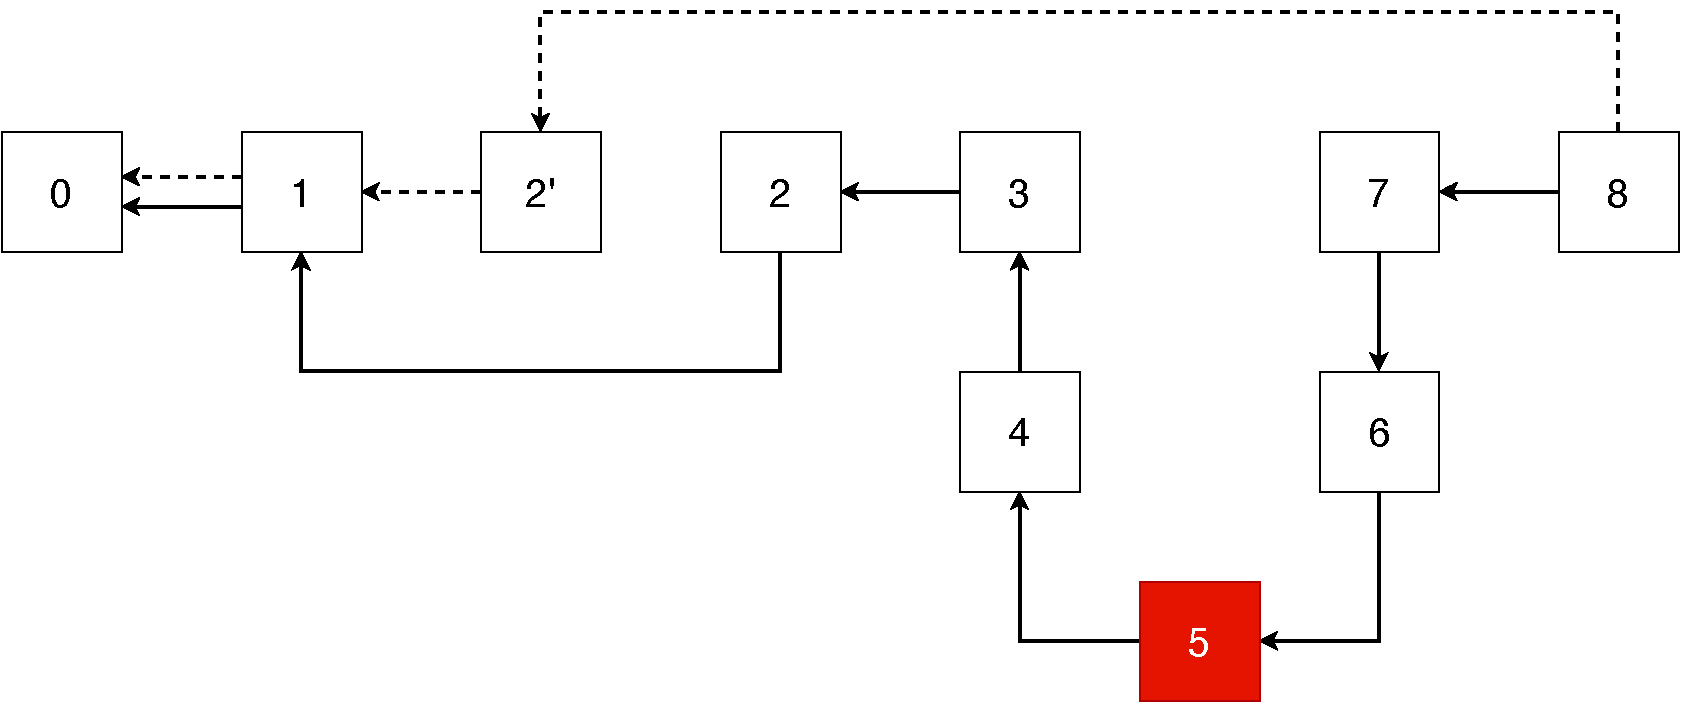
\includegraphics[width=8cm]{./images/DAG_usage.pdf}
    \caption{Combination of multiple proofs in a DAG. The red block is the
        block of interest. Honest proof consists of blocks connected by solid
        lines and adversarial proof by dashed lines. The adversary
        intentionally uses a different set of blocks.}
    \label{figure:DAG_usage}
\end{figure}


This logic is intuitive and efficient to implement in most traditional
programming languages (C++, JAVA, Python, JavaScript, etc). However, as our
analysis proves, such an algorithm cannot be efficiently implemented in
Solidity as is. This is not due to the lack of features, such as the existence
of hashmaps, but because Solidity treats storage differently than traditional
programming languages. In smart contracts, the caller needs to pay in gas for
the execution of operations such as accessing and storing data. Reading from
and writing to persistent memory are very expensive operations in Solidity, as
stated in the Ethereum yellow paper(ref). A summary of gas costs for storage
and memory access if is displayed in Table~\ref{table:ethereum_gas_list}. This
fact was observed by Giorgos et al.\ and was recognized as the bottleneck of
the application.

\begin{table}[]
\centering
\begin{tabular}{@{}llr@{}}
\toprule
\multicolumn{1}{c}{Operation} & \multicolumn{1}{c}{Cost} & \multicolumn{1}{c}{Desc} \\
\midrule
$G_{create}$ & 32000 & Paid for a CREATE operation.\\
$G_{sload}$ & 200 & Paid for a SLOAD operation.\\
$G_{sset}$ & 20000 & Paid for an SSTORE operation.\\
$G_{memory}$ & 3 & Paid words expanding memory.\\
$G_{txdatazero}$ & 4 & Paid for zero byte of data for a transaction.\\
$G_{txdatanonzero}$ & 68 & Paid for non-zero byte of data for a transaction.\\
\end{tabular}
\caption{Ethereum gas list}
\label{table:ethereum_gas_list}
\end{table}


\subsubsection{Solidity Algorithms}

We describe each phase of previous implementation in
Algorithms~\ref{algo:submit_old} and~\ref{algo:contest_old}. We denote
structures that access persistent memory as $struct_{s}$. Note that deleting
from persistent memory is also considered a storage operation.

\begin{algorithm}[H]
    \caption{Submit Event Proof}
    \label{algo:submit_old}
    \KwIn{$proof$, $predicate$}
    \KwData{
        \texttt{array} $proof_{s}$,
        \texttt{hashmap} $DAG_{s}$,
        \texttt{bool} $predicate_{s}$
    }
    require $predicate_{s}$ $=$ $\emptyset$ \\
    require $validInterlink(proof$) \\
    $DAG_{s}$ $\leftarrow$ $DAG_{s}$ $\cup$ $proof$\\
    $proof_{s}$ $\leftarrow$ $proof$\\
    $ancestors_{s}$ $\leftarrow$ $findAncestors(DAG_{s}$)\\
    $predicate_{s}$ $\leftarrow$ $evaluatePredicate(ancestors_{s}$,
    $predicate$)\\
    delete $ancestors_{s}$\\
\end{algorithm}

\begin{algorithm}
    \caption{Submit Contesting Proof}
    \label{algo:contest_old}
    \KwIn{$proof'$, $predicate$}
    \KwData{
        \texttt{array} $proof_{s}$,
        \texttt{hashmap} $DAG_{s}$,
        \texttt{bool} $predicate_{s}$
    }
    require $predicate_{s}$ = $predicate$\\
    $lca$ $\leftarrow$ findLca($proof_{s}$, $proof'$)\\
    require $score(proof’[lca:])$ $>$ $score(proof_{s}[lca:])$ \\
    $DAG_{s}$ $\leftarrow$ $DAG_{s}$ $\cup$ $proof'$\\
    $ancestors_{s}$ $\leftarrow$ $findAncestors(DAG_{s})$\\
    $predicate_{s}$ $\leftarrow$ $evaluatePredicate(ancestors_{s},
    predicate)$\\
    delete $ancestors_{s}$\\
\end{algorithm}



\section{Difficulty}

Describe constant and non-constant difficulty
